%%%%%%%%%%%%%%%%%%%%%%%%%%%%%%%%%%%%%%%%%
% fphw Assignment
% LaTeX Template
% Version 1.0 (27/04/2019)
%
% This template originates from:
% https://www.LaTeXTemplates.com
%
% Authors:
% Class by Felipe Portales-Oliva (f.portales.oliva@gmail.com) with template 
% content and modifications by Vel (vel@LaTeXTemplates.com)
%
% Template (this file) License:
% CC BY-NC-SA 3.0 (http://creativecommons.org/licenses/by-nc-sa/3.0/)
%
%%%%%%%%%%%%%%%%%%%%%%%%%%%%%%%%%%%%%%%%%

%----------------------------------------------------------------------------------------
%	PACKAGES AND OTHER DOCUMENT CONFIGURATIONS
%----------------------------------------------------------------------------------------

\documentclass[
  french,
  % twocolumn,
	10pt, % Default font size, values between 10pt-12pt are allowed
	%letterpaper, % Uncomment for US letter paper size
	%spanish, % Uncomment for Spanish
]{fphw}

\usepackage[fontsize=10.0]{scrextend} % Use this to force the fontsize

%% Commands for numering paragraphs
\renewcommand\thesection{\Roman{section}}
\renewcommand\thesubsection{\thesection.\arabic{subsection}}
\renewcommand*\thesubsubsection{%
  \Roman{section}.\arabic{subsection}.\alph{subsubsection}%
}

 % \usepackage{fancyhdr}
% Template-specific packages
\usepackage{babel}
\usepackage[utf8]{inputenc} % Required for inputting international characters
\usepackage{DejaVuSerifCondensed} 
\usepackage[T1]{fontenc} % Output font encoding for international characters
% \usepackage{mathpazo} % Use the Palatino font
% \usepackage{tgschola} % Use the Palatino font
% \usepackage{Alegreya}
% \renewcommand*\oldstylenums[1]{{\AlegreyaOsF #1}}
% \usepackage{iwona} % Use the Iwona font

\usepackage{fancyvrb}
\usepackage{fvextra}
\newcommand\userinput[1]{\textbf{#1}}
\newcommand\arguments[1]{\textit{#1}}

\usepackage{amsmath}
\usepackage{mathtools}
\usepackage{xfrac} 

\usepackage{graphicx} % Required for including images
\usepackage[textfont=it,font=small]{caption}  %% To manage long captions in images
\usepackage{subcaption}
\captionsetup{justification=centering}

\usepackage{float}
\graphicspath{ {../Images/} }

\usepackage{booktabs} % Required for better horizontal rules in tables

\usepackage{listings} % Required for insertion of code

\usepackage{array} % Required for spacing in tabular environment

\usepackage{enumerate} % To modify the enumerate environment

\usepackage{amssymb}
\usepackage{enumitem}	%% % To modify the itemize bullet character

\newcommand{\tabhead}[1]{{\bfseries#1}}

\usepackage{xcolor}
\usepackage{listings}
\colorlet{mygray}{black!30}
\colorlet{mygreen}{green!60!blue}
\colorlet{mymauve}{red!60!blue}
\lstset{
  backgroundcolor=\color{gray!10},  
  basicstyle=\ttfamily,
  columns=fullflexible,
  breakatwhitespace=false,      
  breaklines=true,                
  captionpos=b,                    
  commentstyle=\color{mygreen}, 
  extendedchars=true,              
  frame=single,                   
  keepspaces=true,             
  keywordstyle=\color{blue},      
  language=c++,                 
  numbers=none,                
  numbersep=5pt,                   
  numberstyle=\tiny\color{blue}, 
  rulecolor=\color{mygray},        
  showspaces=false,               
  showtabs=false,                 
  stepnumber=5,                  
  stringstyle=\color{mymauve},    
  tabsize=3,                      
  title=\lstname                
}

\usepackage[linkcolor=blue,colorlinks=true]{hyperref}
% \usepackage[colorlinks=true,urlcolor=blue]{hyperref}
\hypersetup{citecolor=blue}

\usepackage{cleveref}
\usepackage{siunitx}
\newcommand{\bvec}[1]{\bm{#1}}    %% For vector notation
\newcommand{\myvec}[3]{\begin{pmatrix} #1  \\ #2 \\ #3 \end{pmatrix}}   %% vecteur 3d
\newcommand{\mymat}[9]{\begin{pmatrix} #1 & #2 & #3 \\ #4 & #5 & #6 \\ #7 & #8 &#9 \end{pmatrix}}  %% Matrice 3*3

\renewcommand{\vector}[4]{\begin{pmatrix} #1  \\ #2 \\ #3 \\ #4 \end{pmatrix}}   %% vecteur 3d
% \newcommand{\mymatrix}[16]{\begin{pmatrix} #1 & #2 & #3 & #4 \\ #4 & #6 & #7 & #8 \\ #9 & #10 & #11 & #12 \\ #13 & #14 & #15 & #16 \end{pmatrix}}  %% Matrice 3*3

\newcommand{\hquad}{\hspace{0.5em}} %% Bew command for half quad
\setlength\parindent{0.65cm}	%% To remove all indentations

% \setlength{\parskip}{1em}%
% \setlength\parindent{0pt}

\usepackage[backend=bibtex,style=authoryear,maxnames=2,natbib=true]{biblatex} % Use the bibtex backend with the authoryear citation style (which resembles APA)
\addbibresource{main-bib.bib} % The filename of the bibliography
\usepackage[autostyle=true]{csquotes} % Required to generate language-dependent quotes in the bibliography 
% \renewcommand*{\bibfont}{\tiny} % Pour reduire la taille des references

%----------------------------------------------------------------------------------------
%	ASSIGNMENT INFORMATION
%----------------------------------------------------------------------------------------

\title{Projet SIR} % Assignment title

\author{Roussel Desmond Nzoyem} % Student name

\date{\today} % Due date

\institute{Université de Strasbourg \\ UFR de Mathématiques et Informatique} % Institute or school name

\class{Incertitudes} % Course or class name

\professor{Pr. Frédéric Bertrand} % Professor or teacher in charge of the assignment

%----------------------------------------------------------------------------------------

\begin{document}

% \maketitle % Output the assignment title, created automatically using the information in the custom commands above

%----------------------------------------------------------------------------------------
%	ASSIGNMENT CONTENT - SECTION 1
%----------------------------------------------------------------------------------------

\renewcommand{\abstractname}{Introduction}
\maketitle
\begin{abstract}
  \normalsize
  L'objectif de ce travail est la simulation de l'épidémie de COVID-19 par un modèle de type SIR, dont les paramètres seront estimés principalement par calage déterministe. Nous avons choisi le modèle \textbf{SIRD} (Susceptibles-Infectés-Retirés(ou Rétablis)-Décédés) avec introduction du taux de natalité et de mortalité général de la population. Le modèle a été implémenté en langage Python avant d'être intégré à la librairie de calcul d'incertitudes \textbf{OpenTurns}. Ce modèle comporte neuf paramètres (y compris les conditions initiales) dont les lois de probabilités ont été estimées en utilisant les observations faites au \textbf{Cameroun} entre le 06 mars et le 14 juin 2020. Après une comparaison des résultats avec ceux obtenus dans une étude faite par \textbf{Nguemdjo et al.}, nous avons réussi à prédire l'évolution de l'épidémie. Les analyses de sensibilité par développement de Taylor et par calcul des indices de Sobol ont permis d'extraire des indications sur la limitation des ravages causés par l'épidémie au Cameroun.
\end{abstract}


\section{Modélisation mathématique}

D'entrée, le modèle choisi est limité par les données auxquelles on aura accès pour la partie 2 de cette étude (il s'agira de l'estimation des paramètres). Nous avons opté pour le modèle SIRD (\cite{Kaggle}) avec ajout du taux de natalité $\mu$ et du taux de mortalité $\nu$ de la population générale (\cite{CNRS})\footnote{Attention, dans l'article du CNRS qui a inspirée ce modèle, les définitions de $\mu$ et $\nu$ sont inversées. Précisons aussi que dans cet article, l'introduction de la natalité et de la mortalité se fait à travers l'étude du modèle SEIR.}. 

\subsection{Le modèle SIRD}

Commençons par décrire le modèle SIRD fréquemment rencontré dans la littérature. Nous sommes déjà familier avec le modèle classique SIR qui décrit respectivement les populations Susceptibles de contacter les virus, celles Infectées par le virus, et celles Retirées de l'étude. Dans le modèle SIR, les personnes Retirées (R) sont supposées soit guéries (et immunisées), soit décédés. Cela dit, les organismes d'agrégation de données comptent généralement les populations guéries et décédés séparément. On obtient alors le modèle SIRD dans lequel le R est mis pour Retirés\footnote{Bien que ce terme désigne à présent les population Rétablies, nous utiliserons le terme "Retirés" pour raison de concordance avec le modèle SIR classique.} (ou Rétablis), et le D mis pour Décédés. Ce modèle est décrit à la \cref{fig:SIRD1}.
\begin{figure}[H]
  \centering
  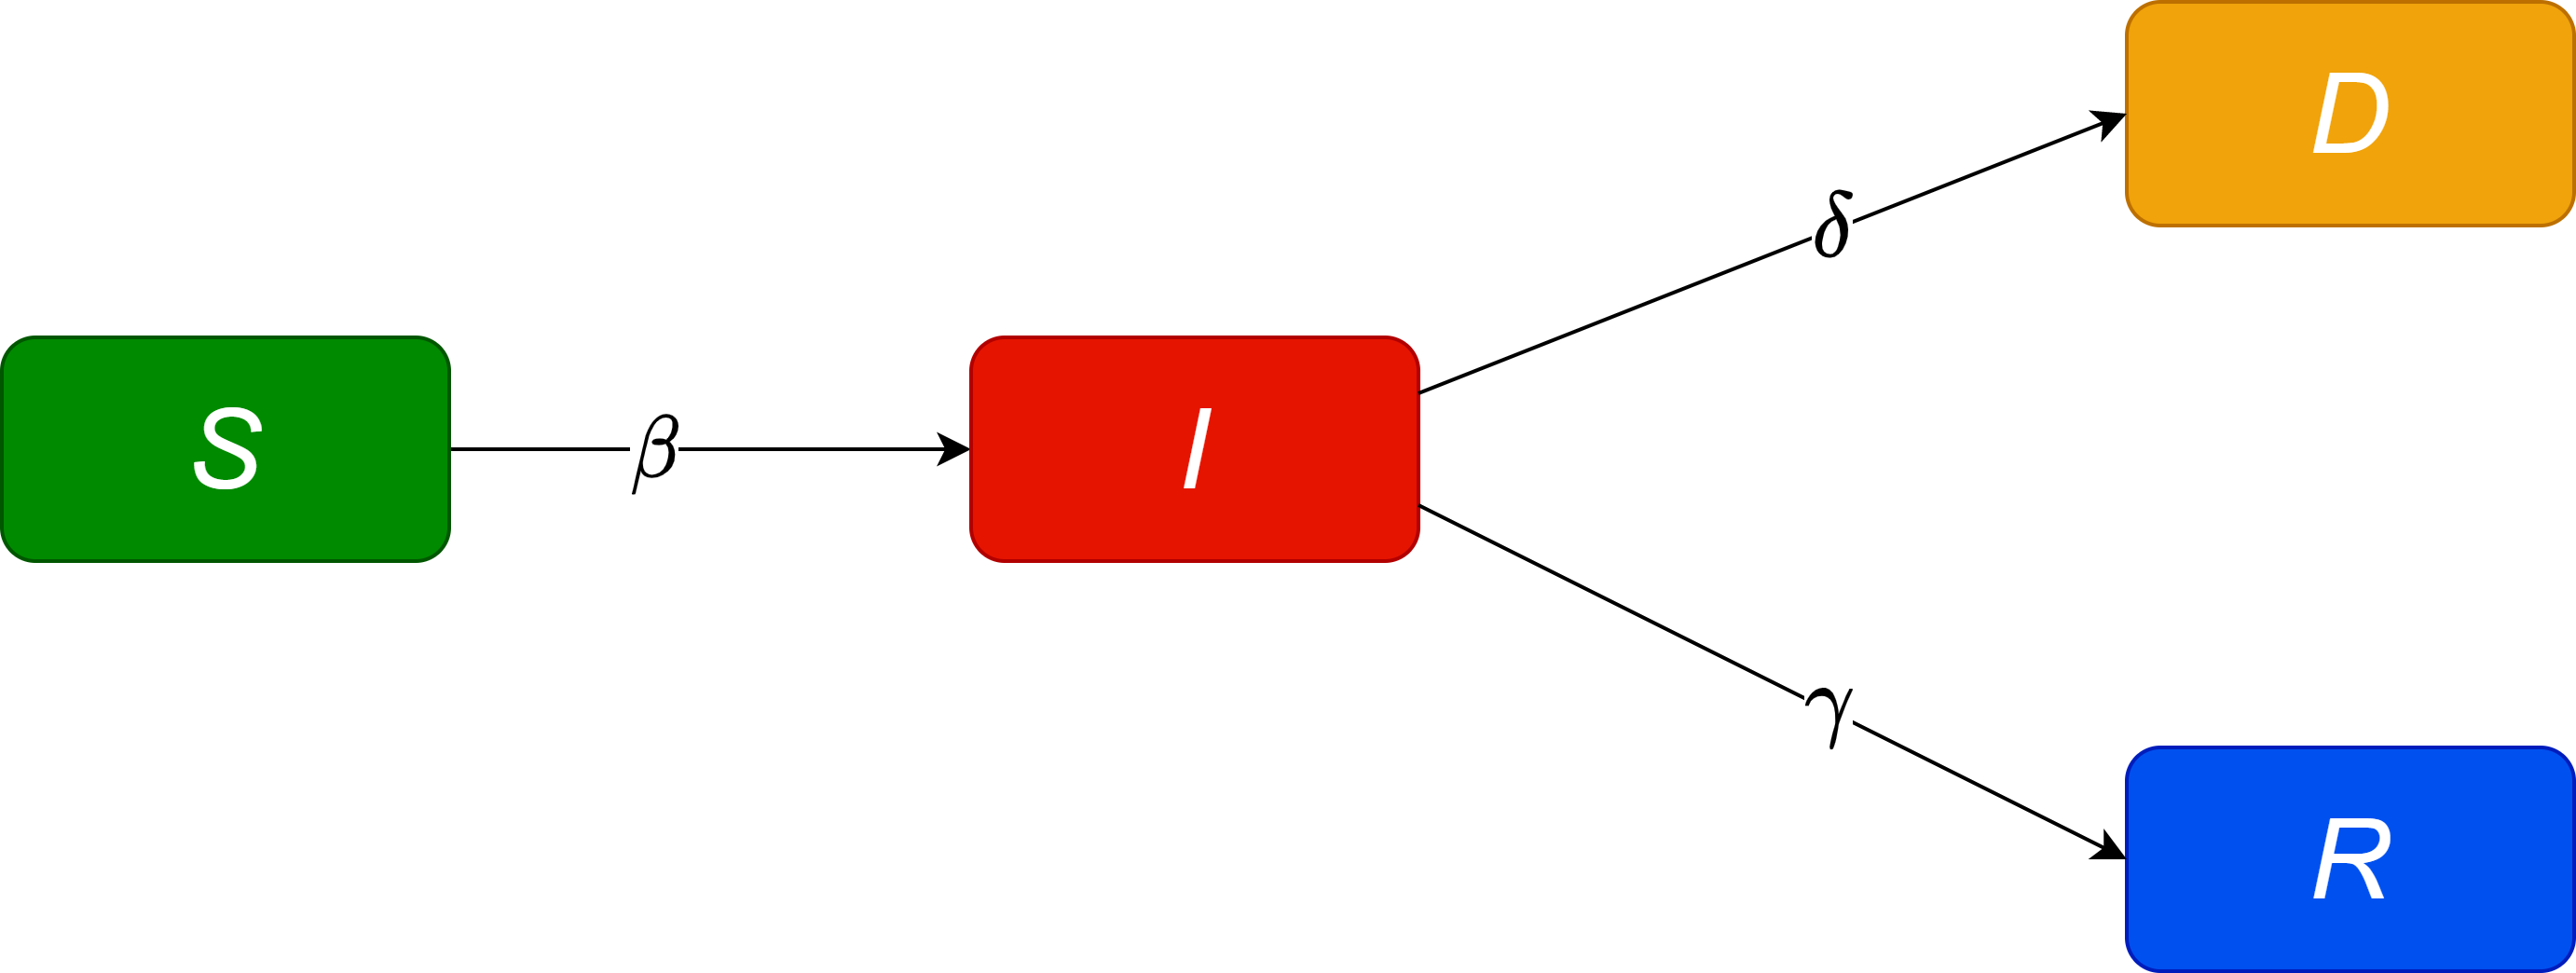
\includegraphics[width=7cm]{SIRD1.png}
  \caption{Illustration du modèle SIRD. $\beta$ représente la proportion de personnes saines (susceptibles) qui deviennent infectées après un contact avec une personne infectée. Autrement dit, il s'agit du taux de transmission du virus. $\gamma$ désigne le taux de guérison, et $\delta$ le taux de mortalité lié au virus.}
  \label{fig:SIRD1}
\end{figure}


\subsection{Le modèle SIRD avec natalité et mortalité}

Le modèle SIRD suppose que la population totale reste constante durant l'épidémie, ce qui est rarement le cas. Nous décidons donc de complexifié le modèle SIRD en y ajoutant les taux de natalité $\mu$ et du taux de mortalité $\nu$ liés à la population\footnote{Notons que ce taux de mortalité n'est pas lié au virus.}. Dans la suite de ce rapport, nous désignerons ce modèle par SIRD*. Le schéma suivant illustre la dynamique dudit système.
\begin{figure}[H]
  \centering
  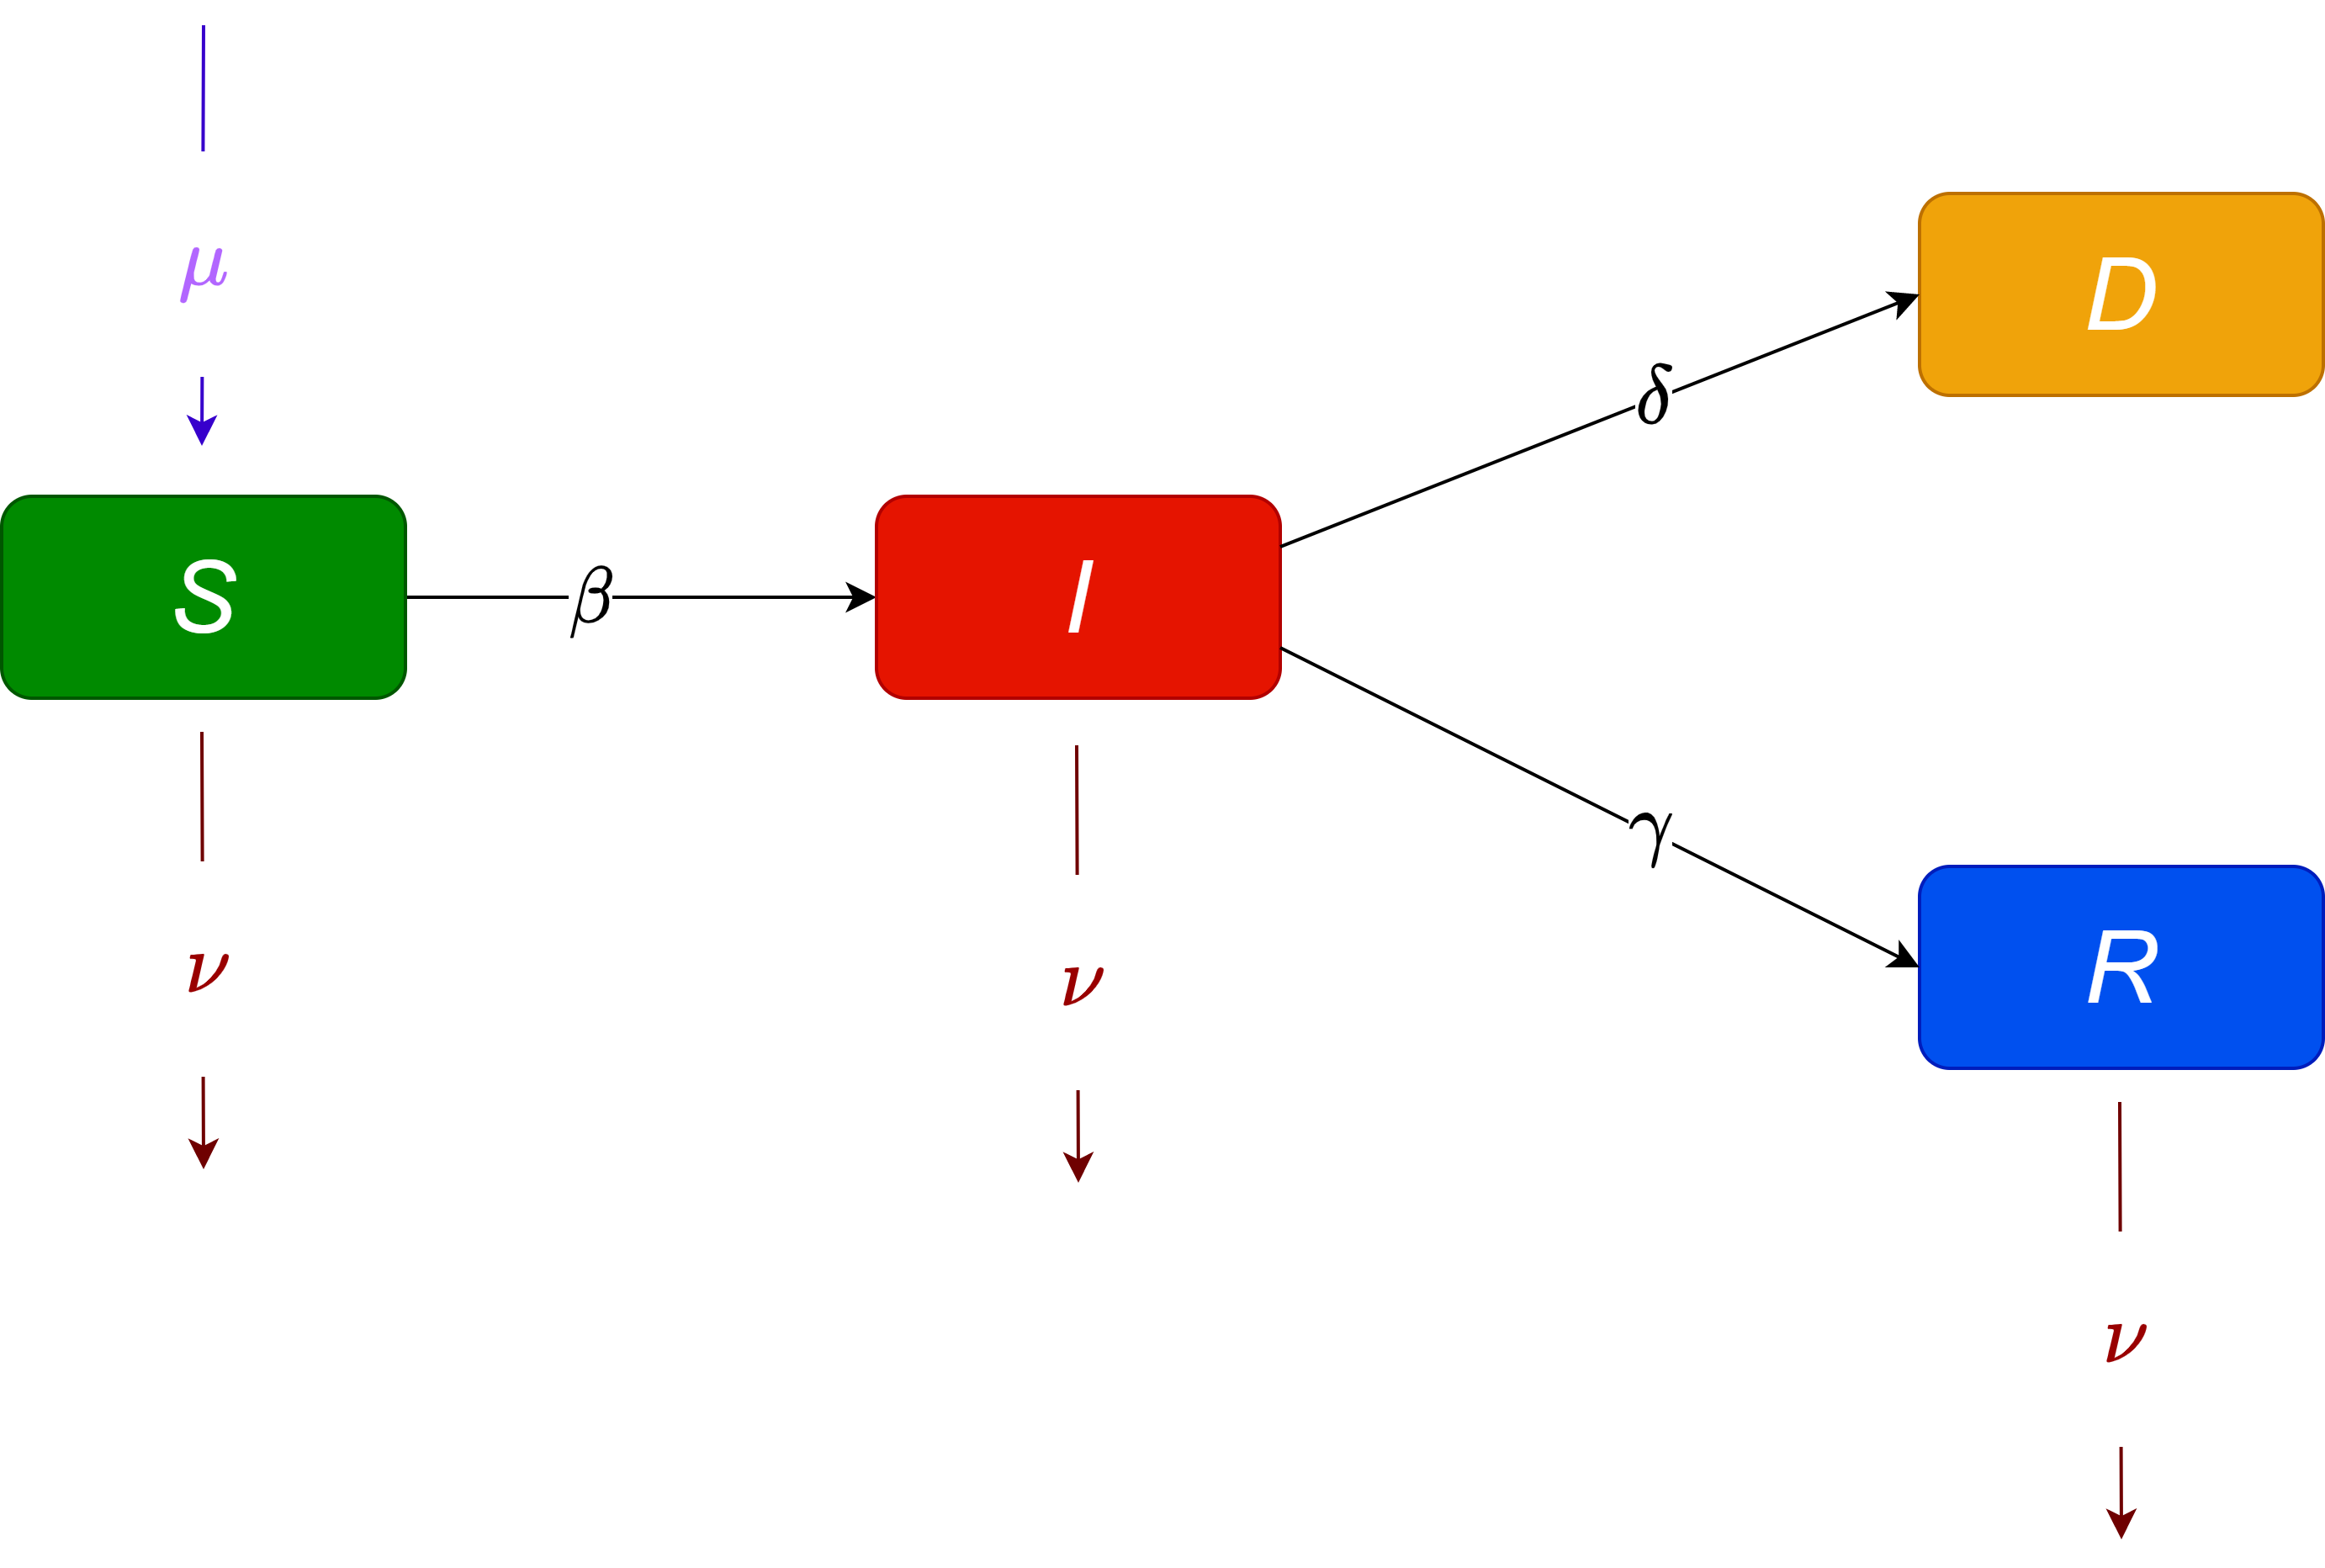
\includegraphics[width=7cm]{SIRD2.png}
  \caption{Illustration du modèle SIRD avec ajout du taux de natalité $\mu$ et du taux de mortalité $\nu$ de la population. Notons que contrairement à l'article du CNRS (\cite{CNRS}) qui a inspirée ce modèle, les definitions de $\mu$ et $\nu$ sont inversées.}
  \label{fig:SIRD2}
\end{figure}
Notons que les personnes qui naissent sont bien évidemment non décédés, d'où l'ajout d'une somme (pondéré par le taux de natalité) des populations saines (S), infectées (I), et retirées (R) aux populations susceptibles (S). De manière similaire, les populations décédées (de cause non liée au virus) seront soustraites des populations S, I, et R. Cela nous donne le système d'EDO suivant\footnote{Pour plus de clarté, les dépendances des variables $S, I, R, D$ ou $N$ en fonction de $t$ n'ont pas été précisées dans ces équations.} :
\begin{align*}
  \tag{$\mathcal{SIRD^*}$}
  \begin{dcases}    
  & \frac{\mathrm{d}S}{\mathrm{d}t}= - \beta \frac{S I}{N}  + \mu (S+I+R) - \nu S \\
  & \frac{\mathrm{d}I}{\mathrm{d}t}= \beta \frac{S I}{N} - (\gamma + \delta) I - \nu I \\
  & \frac{\mathrm{d}R}{\mathrm{d}t}= \gamma I - \nu R \\
  & \frac{\mathrm{d}D}{\mathrm{d}t}= \delta I
  \end{dcases}
\end{align*}

Remarquons que contrairement aux modèles SIR et SIRD, la population totale $N$ dans le modèle SIRD* n'est pas forcément constante. En effet, on a 
\begin{align*}
  \frac{\mathrm{d}N}{\mathrm{d}t} &= \frac{\mathrm{d}(S+I+R+D)}{\mathrm{d}t} \\
  &= \mu (S+I+R) -\nu (S+I+R) \\
  &=  (\mu -\nu) (S+I+R)
\end{align*}
et donc
\begin{itemize}
  \item Si $\mu > \nu$, la population totale augmente
  \item Si $\mu = \nu$, la population totale est constante
  \item Si $\mu < \nu$, la population totale diminue
\end{itemize}

Concernant le taux de reproduction du virus, on se focalise sur l'EDO sur le nombre d'infectés (I) dans le système ($\mathcal{SIRD^*}$) pour trouver :
$$\mathcal{R}_0 = \frac{\beta}{\gamma + \delta + \nu}$$
On sait que si :
\begin{itemize}
  \item $\mathcal{R}_0 > 1$, le virus se propage dans la population\footnote{La probabilité d'avoir une épidémie n'est cependant pas garantie d'après \cite[p.4]{Nguemdjo}.}
  \item $\mathcal{R}_0 \leq 1$, la propagation du virus va s'arrêter au bout d'un moment
\end{itemize}

C'est donc ce modèle que nous avons implémenté en Python par un schéma de Runge-Kutta d'ordre 4. Nous présentons ci-bas quelques résultats de simulation.
\begin{figure}[H]
	\centering
	\begin{subfigure}{0.48\textwidth}
		\centering
		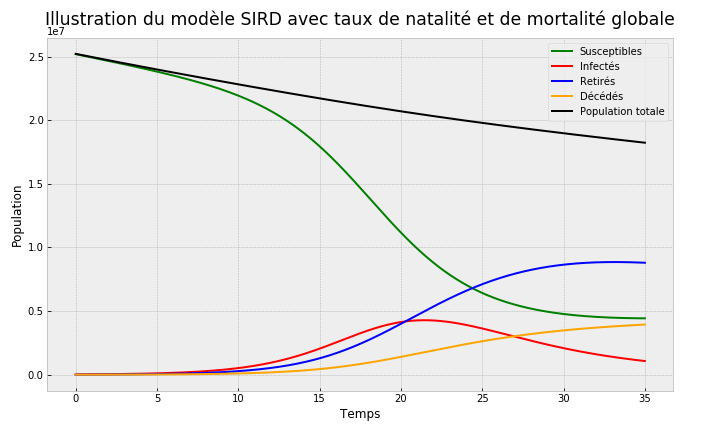
\includegraphics[width=\textwidth]{Simu1.png}
	  \caption{$\mu = 0.02 \leq 0.03 = \nu$}
  \label{fig:simu1}
	\end{subfigure}
	\begin{subfigure}{0.48\textwidth}
		\centering
		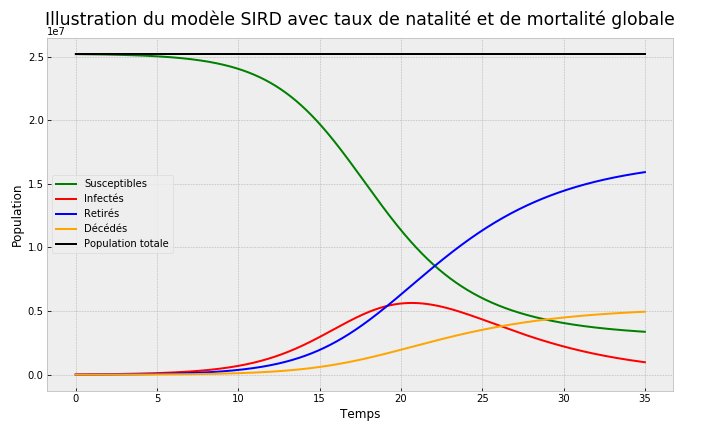
\includegraphics[width=\textwidth]{Simu2.png}
	  \caption{$\mu = \nu = 0$}
  \label{fig:simu2}
	\end{subfigure}
	\caption{Illustrations des résultats de l'implémentation du modèle SIR avec les coefficients $\beta = 0.615, \gamma=0.193, \delta = 0.06$ fixés. Les conditions initiales sont $S_0 = 25216237-2e4, I_0=2e4, R_0=0, D_0=0$, et le temps de simulation est de $T=35$ jours. Remarquons que la figure (b) permet de revenir à un modèle SIRD classique, où la population totale reste constante.}
	\label{fig:simu}
\end{figure}



%----------------------------------------------------------------------------------------
%	ASSIGNMENT CONTENT - SECTION 2
%----------------------------------------------------------------------------------------
\section{Estimation des paramètres}

Dans cette section, nous allons estimer les lois de probabilité suivies par cinq des paramètres du modèle. Il s'agit d'estimer les distributions sur $\beta, \gamma, \delta, \mu, $ et $\nu$. Pour ce faire, nous devons obtenir des donnés observées sur une population. Nous choisissons naturellement le cas du Cameroun (CMR), où le premier cas d'infection a été constaté le 06 mars 2020. 

\subsection{Création des entrées-sorties observées}

En janvier 2020, au tout début de l'éruption du Coronavirus, le CSSE\footnote{Center for Systems Science and Engineering} de l'Université Johns Hopkins (\cite{JHU}) s'est mise à regrouper des informations\footnote{Ces données sont à l'échelle internationale et proviennent de plusieurs sources fiables.} visualisables \href{https://www.arcgis.com/apps/opsdashboard/index.html#/bda7594740fd40299423467b48e9ecf6}{sur ce site}. Les données correspondantes sont conservées sur un dépôt GitHub (\cite{GitHub}) mis à jour quotidiennement. Nous y avons récupéré les informations liées au Cameroun sur la période du 22 janvier 2020 au 10 janvier 2021. Ces informations sont obtenues sous forme de trois séries temporelles (cf. \cref{fig:RawData}) : 
\begin{itemize}
  \item le nombre de cas confirmés ("confirmed")
  \item le nombre de cas décédés ("deaths")
  \item le nombre de cas rétablis ("recovered")
\end{itemize}

\begin{figure}[H]
	\centering
	\begin{subfigure}{0.32\textwidth}
		\centering
		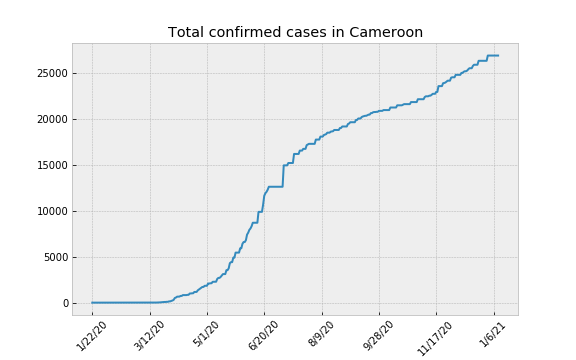
\includegraphics[width=\textwidth]{Confirmed.png}
	  \caption{Cas confirmés}
  \label{fig:confirmed}
	\end{subfigure}
	\begin{subfigure}{0.32\textwidth}
		\centering
		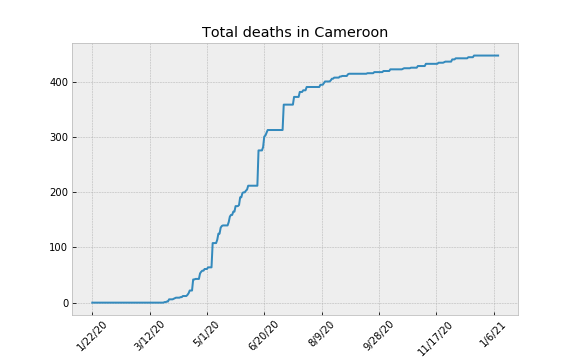
\includegraphics[width=\textwidth]{Deaths.png}
	  \caption{Cas décédés}
  \label{fig:deaths}
  \end{subfigure}
	\begin{subfigure}{0.32\textwidth}
		\centering
		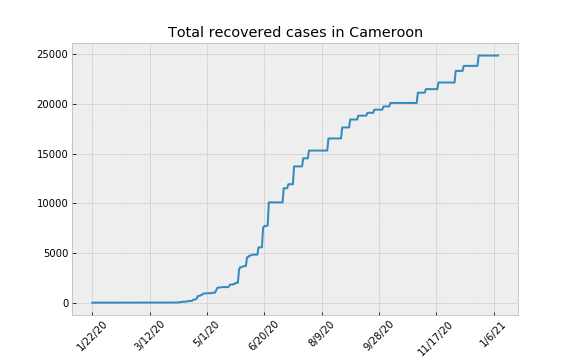
\includegraphics[width=\textwidth]{Recovered.png}
	  \caption{Cas rétablis}
  \label{fig:recovered}
	\end{subfigure}
	\caption{Illustration des données brutes obtenues de la base de données de l'Université Johns Hopkins concernant l'évolution du COVID-19 au Cameroun du 22 janvier 2020 au 10 janvier 2021. Les effectifs présentés sur cette figure sont des effectifs cumulés.}
	\label{fig:RawData}
\end{figure}
 Une fois les données brutes obtenues, il nous faut les classer en fonction des catégories qui sont intéressantes pour notre modèle SIRD*. Aucun recensement de population n'ayant eu lieu entre les dates d'observation, la population totale du Cameroun sera supposée constate $N=25,216,237$. On a les relations suivantes (\cref{fig:pretreated}) :
 \begin{itemize}
   \item Décédés = Nombre de cas décédés
   \item Retirés = Nombre de cas rétablis
   \item Infectés = Nombre de cas confirmés - détectés - rétablis
   \item Susceptibles = Population totale - Nombre de cas confirmés
 \end{itemize} 

\begin{figure}[H]
  \centering
  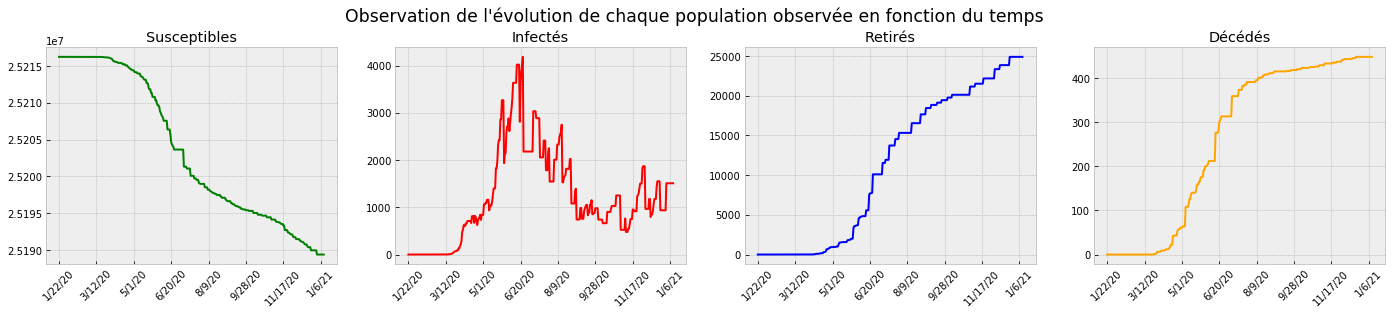
\includegraphics[width=\linewidth]{pretreated.png}
  \caption{Illustration des données prétraitées sur la période du 22 janvier 2020 au 10 janvier 2021 au Cameroun.}
  \label{fig:pretreated}
\end{figure}

Une fois les données prétraitées et classées par catégories, on peut créer les entrées et les sorties observées. Mais avant, il faut choisir une fenêtre dans laquelle faire notre étude. Comme mentionné plus haut, le premier cas de COVID-19 a été détecté au Cameroun le 06 mars 2020 ; notre étude débutera donc à cette date, et s'achèvera 100 jours plus tard, soit le 14 juin 2020. Dans cette fenêtre, on prend des observations correspondant à des simulations sur 15 jours chacune. On peut en extraire 85 qui soient valides. En résumé, si $X(t)$ correspondant à l'état du système au temps $t$, alors l'entrée observée vaut $X(t)$ et la sortie observée correspondante vaut $X(t+15)$. Cela correspond au code ci-bas, dont le résultat est visualisé à la \cref{fig:treated}.

\begin{lstlisting}[language=Python, caption={Code de génération des entrées-sorties afin d'effectuer l'estimation des paramètres. Les données S, I, R, et D correspondent à ce qui est observé à la \cref{fig:pretreated}.},breaklines]
  inputs = np.zeros((85, 4))
  outputs = np.zeros((85, 4))
  for k in range(85):
      inputs[k] = np.array([S[k], I[k], R[k], D[k]])
      outputs[k] = np.array([S[k+15], I[k+15], R[k+15], D[k+15]])
\end{lstlisting}  

\begin{figure}[H]
  \centering
  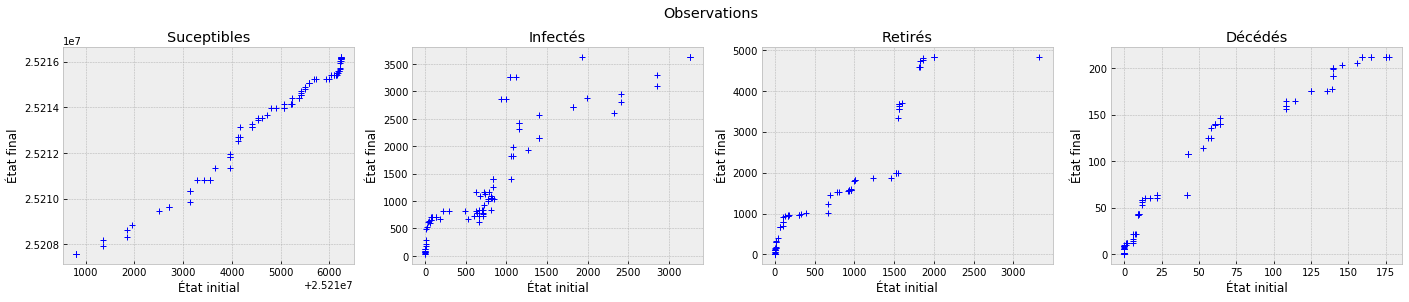
\includegraphics[width=\linewidth]{treated.png}
  \caption{Illustration des données traitées observées sur la période du 06 mars au 14 juin 2020. Ces données seront utilisées pour l'estimation des paramètres. Observons que dû à la faible taille de la simulation (15 jours) à l'intérieur de la fenêtre d'étude, ces données ont une tendance linéaire que nous exploiterons dans la suite. }
  \label{fig:treated}
\end{figure}

\subsection{Estimation des paramètres par calage}

Maintenant que nous avons les données observées, nous pouvons estimer les paramètres qui s'accordent le mieux avec ces données. Pour cela, on se sert d'OpenTurns. Tout d'abord, on crée un objet de type $\verb|PythonFunction|$ pour introduire note modèle SIRD* (implémenté en Python) dans OpenTurns. Ensuite, nous nous servons de la classe $\verb|LinearLeastSquaresCalibration|$ pour estimer les paramètres $\beta, \gamma, \delta, \mu,$ et $\nu$. La décision d'utiliser cet estimateur vient de la tendance linéaire des données observées à la \cref{fig:treated}. Cet estimateur linéarise le modèle et minimise la distance aux données observées\footnote{Au sens des moindres carrés.}, ceci autour d'un état (nommé "prior") que nous choisirons raisonnablement égale à $\verb|[0.467,0.4,0.001,0.0001,0.0001]|$\footnote{En réalité, l'état "prior" a été cherché manuellement, de façon à correspondre à au moins une observation.}. L'estimation des lois de probabilités de ces cinq paramètres produit les lois normales dont les moyennes, les écarts types, les valeurs supérieures et inférieurs des intervalles de confiance (CI) à 95 \% sont présentées dans le tableau ci-après.

\begin{table}[h!]
  \centering
  \begin{tabular}{c c c c c c}
      \toprule
      \tabhead{Paramètre} & \tabhead{Valeur de référence} & \tabhead{Moyenne} & \tabhead{Écart type} & \tabhead{Inf CI} & \tabhead{Sup CI} \\
      \midrule
      \tabhead{$\beta$} & 0.4670 & 0.4503 & 0.0041 & 0.4192 & 0.4813 \\
      \tabhead{$\gamma$} & 0.4000 & 0.3670 & 0.0041 & 0.3353 & 0.3987 \\
      \tabhead{$\delta$} & 0.0010 & 0.0057 & 0.0028 & -0.0155 & 0.0269 \\
      \tabhead{$\mu$} & 0.0001 & 0.0565 & 0.0019 & 0.0423 & 0.0707 \\
      \tabhead{$\nu$} & 0.0001 & 0.0565 & 0.0019 & 0.0423 & 0.0707 \\
      \bottomrule
  \end{tabular}
  \caption{Résultats de l'estimation des paramètres. La valeur de référence indiquées est la valeur "prior", celle donnée à l'estimateur linéaire de moindres carrés d'OpenTurns. Les quatre colonnes d'après correspondent aux valeurs dites "posterior", celles qu'on obtient après l'estimation.}
  \label{tab:params}
\end{table}

\begin{table}[h!]
  \centering
  \begin{tabular}{c| c c c c c}
      \toprule
      & \tabhead{$\beta$} & \tabhead{$\gamma$} & \tabhead{$\delta$} & \tabhead{$\mu$} & \tabhead{$\nu$} \\
      \midrule
      \tabhead{$\beta$} & 1 & 0.5705 & 0.2350 & 0.5248 & 0.5248 \\
      \tabhead{$\gamma$} & 0.5705 & 1 & -0.2793 & -0.0712 & -0.0712 \\
      \tabhead{$\delta$} & 0.2350 & -0.2793 & 1 & -0.2161 & -0.2161 \\
      \tabhead{$\mu$} & 0.5248 & -0.0712 & -0.2161 & 1 & 1 \\
      \tabhead{$\nu$} & 0.5248 & -0.0712 & -0.2161 & 1 & 1 \\
      \bottomrule
  \end{tabular}
  \caption{Matrice de corrélation après l'estimation des différents paramètres. Cette matrice ne nous sert qu'à des fins d'analyse, et nous considérons ces cinq paramètres comme indépendants dans la suite.}
  \label{tab:cor}
\end{table}

\noindent Il est intéressant de constater que l'estimation n'est pas aberrante, de par le fait que les paramètres $\mu$ et $\nu$ sont quasiment identiques en lois (cf. \cref{tab:params}), et parfaitement corrélés après calage (cf. \cref{tab:cor}), ce qui découle de la constance de la population globale durant l'expérience. De façon visuelle, notre processus d'estimation des paramètres est présenté à la \cref{fig:priorpost}.

\begin{figure}[h]
  \centering
  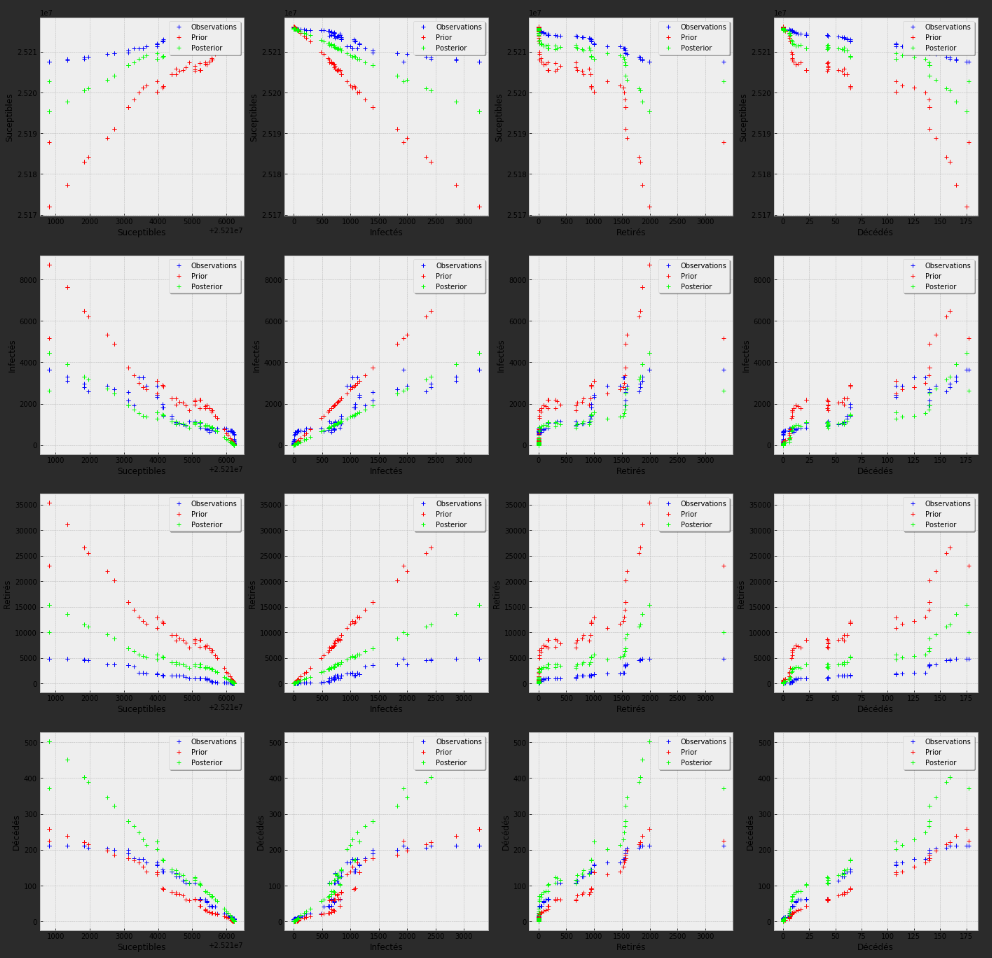
\includegraphics[width=\linewidth]{priorpost.png}
  \caption{Visualisation des états "prior" et "posterior" pour l'estimation des paramètres. On observe bien que les états "posterior" sont globalement plus proche des observations que les états "prior". Notons que ceci n'est pas seulement le cas pour le figures sur la diagonale.}
  \label{fig:priorpost}
\end{figure}

\vspace*{0.6cm}

Notons qu'une étude très similaire à la nôtre a été effectuée par Nguemdjo et al., et publiée en août 2020. Également sur la thématique de la prédiction de l'évolution du COVID-19 au Cameroun, cette étude s'est servie d'un modèle SIR et s'est focalisé sur la fenêtre du 06 mars 2020 au 10 avril 2020. Ses paramètres, obtenus à partir d'un estimateur par maximum de vraisemblance, sont présentés ci-bas.   

\begin{figure}[H]
  \centering
  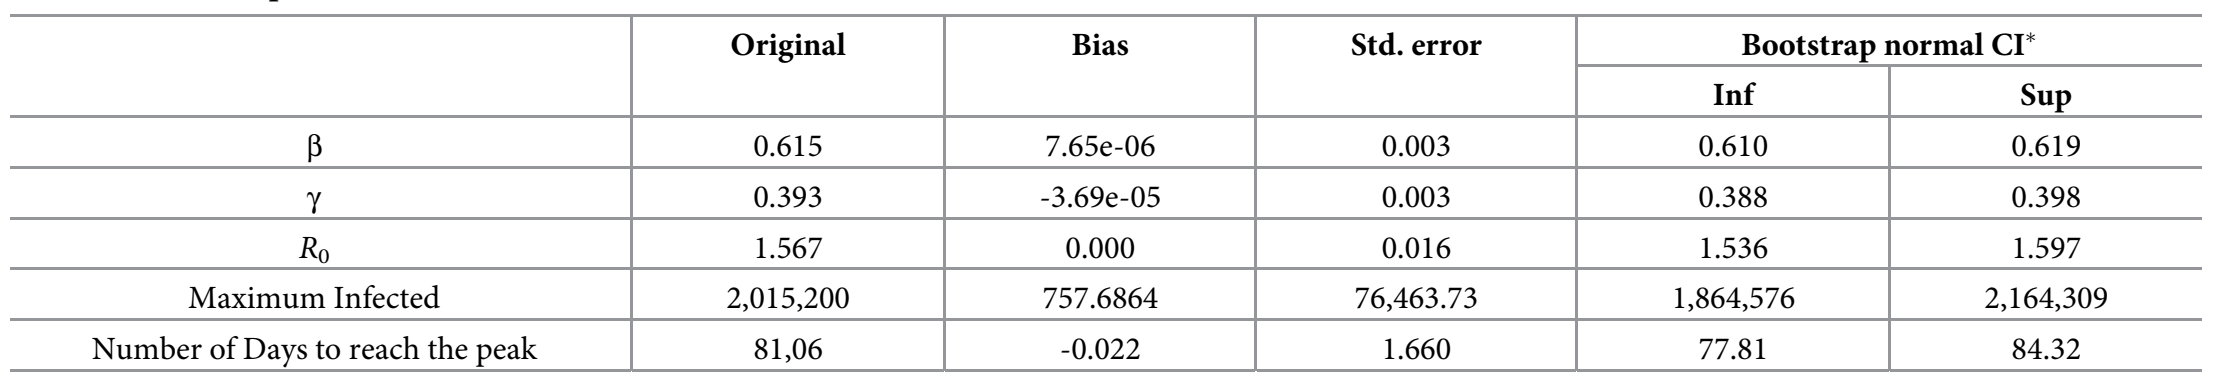
\includegraphics[width=\linewidth]{nguemdjo.png}
  \caption{Résultats obtenus par Nguemdjo et al. sur l'estimation des paramètres d'un modèle SIR (du 06 mars au 10 avril 2020) pour modéliser l'évolution du COVID-19 au Cameroun (\cite[p.4]{Nguemdjo}).}
  \label{fig:Nguemdjo}
\end{figure}

\noindent Remarquons que les résultats ci-hauts (cf. \cref{fig:Nguemdjo}) diffèrent assez largement des nôtres (cf. \cref{tab:params}), pour les paramètres $\beta$ et $\gamma$. En particulier le taux de propagation du virus $\beta$ est considérablement plus bas chez nous. Cette différence s'explique principalement par le fait que la fenêtre d'étude que nous avons choisi (du 06 mars au 14 juin 2020) s'achève juste avant le pic de l'épidémie (cf. \cref{fig:pretreated}), qui correspond à un ralentissement des contaminations, d'où la diminution de $\beta$. En plus, le gouvernement Camerounais a eu le temps de renforcer ses mesures de confinement entre le 10 avril et le 14 juin 2020, ce qui a réduit le taux de propagation du virus \footnote{Dans le code fourni avec ce rapport, il est possible de choisir la même fenêtre d'étude que Nguemdjo et al., même si ce faisant, nous réduisons considérablement la taille des données observées, causant une perte de précision lors de l'estimation des paramètres.}.

\subsection{Analyse de sensibilité}

Nous allons effectuer une analyse de sensibilité de notre modèle SIRD*. En plus des paramètres étudiés dans la partie précédente, nous décidons ici d'analyser aussi l'effet des paramètres initiaux sur le modèle. En résumé, nous analyserons la sensibilité de $S, I, R$ et $D$ par rapport aux paramètres $\beta, \gamma, \delta, \mu, \nu, S_0, I_0, R_0, $et $D_0$. Nous devons au préalable obtenir les distributions de chacun de ces paramètres.

Les cinq premiers paramètres $\beta, \gamma, \delta, \mu, \nu$ ont été estimés dans la section précédente. Leurs loi de probabilités correspondrons à des lois normales dont les moyennes et les écarts-types sont présentées dans le \cref{tab:params} \footnote{Notons que dans le code fourni avec ce rapport, il s'agit des lois marginales de la distribution qui nous est retournée par l'estimateur linéaire décrit à la section précédente.}. En ce qui concerne les conditions initiales $S_0, I_0, R_0,$et $D_0$, elles suivent naturellement les même lois que $S, I, R,$et $D$. En observant la \cref{fig:pretreated} sur la duré du 06 mars au 14 juin 2020, on constate qu'on peut approximer ces lois par des lois Beta. On implémente cela dans OpenTruns et on obtient le résultat du \cref{tab:init}. Le QQ-plot de la \cref{fig:qqplots} confirme effectivement notre choix d'utiliser des lois Beta.
\begin{table}[h!]
  \centering
  \begin{tabular}{c c c c c}
      \toprule
      \tabhead{Paramètre} & \tabhead{alpha} & \tabhead{beta} & \tabhead{a} & \tabhead{b} \\
      \midrule
      \tabhead{$S_0$} & 0.9460 & 0.3721 & 2.52075e+07 & 2.52163e+07 \\
      \tabhead{$I_0$} & 0.4778 & 1.0105 & -34.6078 & 3668.61 \\
      \tabhead{$R_0$} & 0.2528 & 0.7599 & -47.4118 & 4883.41  \\
      \tabhead{$D_0$} & 0.2850 & 0.4967 & -2.07843 & 214.078 \\
      \bottomrule
  \end{tabular}
  \caption{Estimation de lois Beta suivi par les paramètres initiaux par intuition au vu des observations de la \cref{fig:pretreated}.}
  \label{tab:init}
\end{table}

\begin{figure}[H]
  \centering
  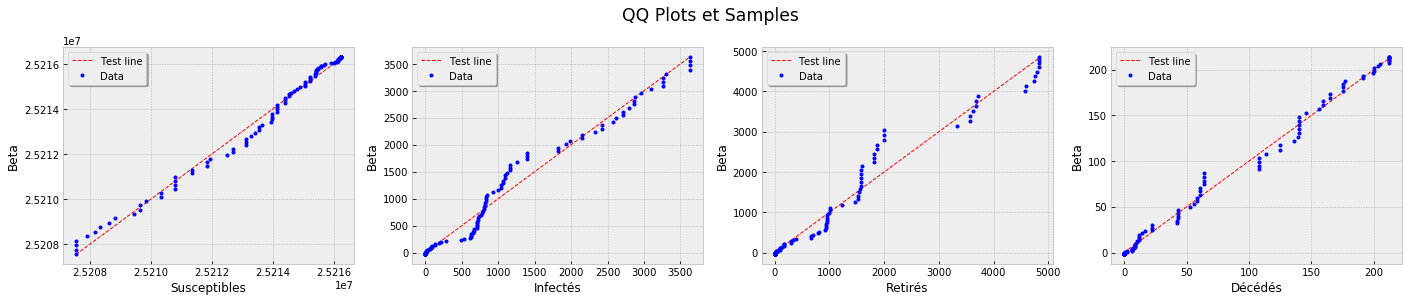
\includegraphics[width=\linewidth]{qqplots.png}
  \caption{Confirmation du choix des lois Beta pour les conditions initiales à travers des QQ-plots.}
  \label{fig:qqplots}
\end{figure}

Connaissant les lois suivies par tout les paramètre en entré du nôtre modèle SIRD*, nous pouvons effectuer les analyses de sensibilité voulues. Nous commençons par une analyse de sensibilité par \textbf{développement de Taylor} au premier ordre. On obtient les facteurs d'importance ci-bas. 
\begin{figure}[H]
  \centering
  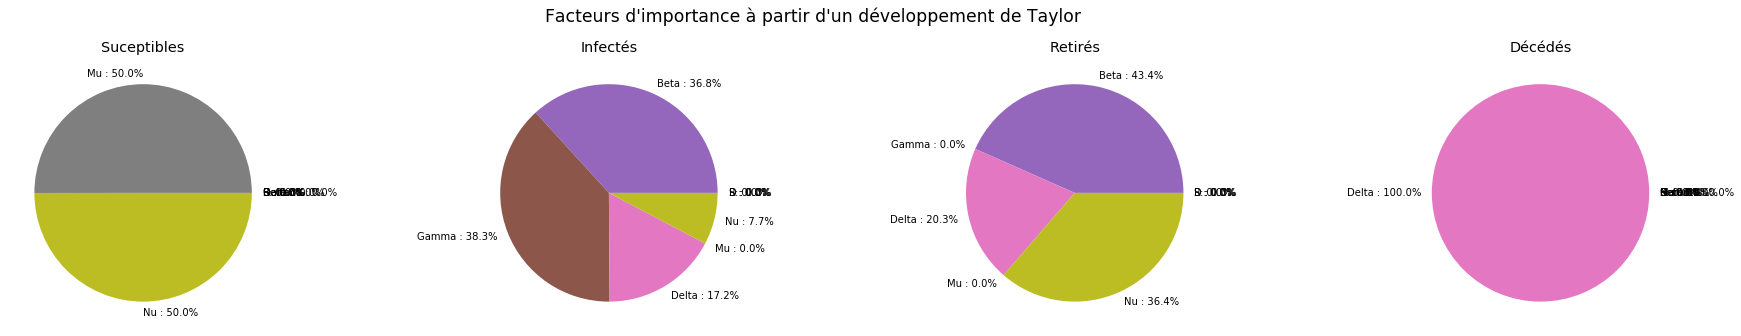
\includegraphics[width=\linewidth]{taylor.png}
  \caption{Analyse de sensibilité par développement de Taylor au premier ordre. On constate que les conditions initiales n'influent pas sur les sorties, ce qui est dû au caractère linéaire de ce développement limité.}
  \label{fig:taylor}
\end{figure}

Ensuite, nous faisons une analyse de sensibilité par calcul des \textbf{indices de Sobol} au premier ordre. Les résultats obtenus sont présentés ci-bas\footnote{Le lecteur est redirigé vers le code accompagnant ce rapport pour les valeurs exactes de ces indices.}.
\begin{figure}[H]
  \centering
  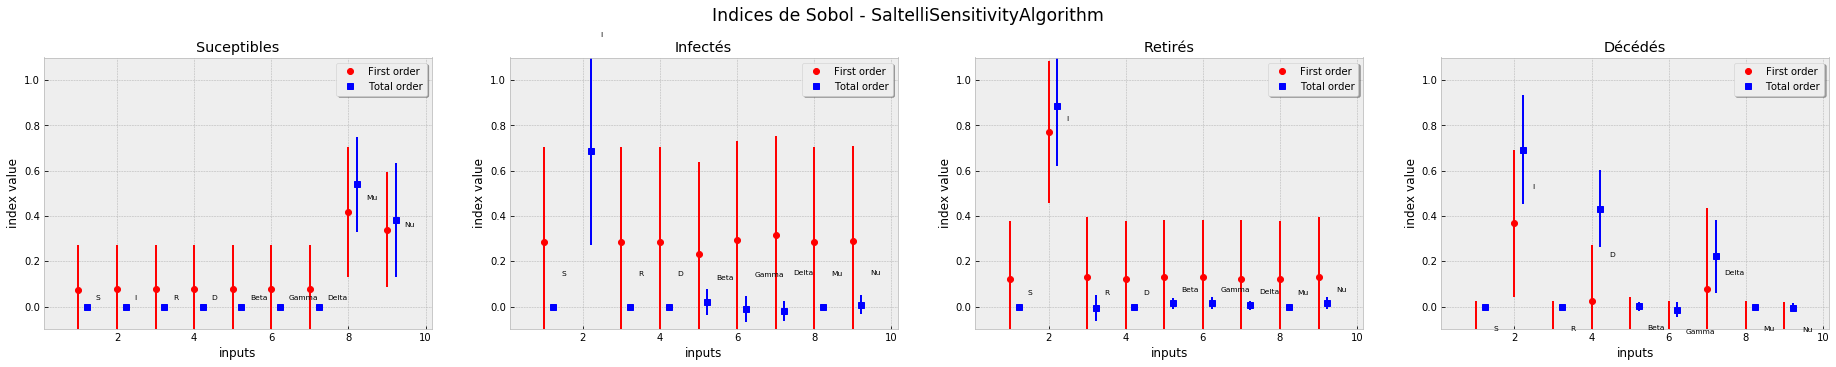
\includegraphics[width=\linewidth]{sobol.png}
  \caption{Analyse de sensibilité par calcul des indices de Sobol au premier ordre et totaux. Remarquons qu'en général, l'indice du premier ordre est différent de l'indice total correspondant, indiquant que les variables étudiés interagissent entre elles, comme nous l'avons montré au \cref{tab:cor}.}
  \label{fig:sobol}
\end{figure}

En analysant les \cref{fig:taylor,fig:sobol} ci-haut, on constate que les paramètres les plus influents sur le nombre de cas susceptible dans la population Camerounaise sont ses taux de natalité $\mu$ et de mortalité $\nu$. Le paramètre le plus influent sur le nombre d'infectés qu'on obtient à la fin d'une simulation est le nombre d'infectés initial. Ce même nombre est crucial pour la détermination des nombres finaux de guéris et de décédés. Remarquons aussi que le nombre de décédés est grandement influencé par plusieurs paramètres, parmi lesquels le taux de mortalité du virus $\delta$.   


%----------------------------------------------------------------------------------------
%	ASSIGNMENT CONTENT - SECTION 3
%----------------------------------------------------------------------------------------
\section{Prédiction de l'évolution de l'épidémie}

Pour prédire l'évolution du virus, nous calculons la distribution suivie par son taux de reproduction $\mathcal{R}_0 = \frac{\beta}{\gamma + \delta + \nu}$. Nous rappelons que les paramètres suivis par les lois $\beta, \gamma, \delta, $ et $\nu$ ont été estimés dans la partie 2 de ce rapport. La densité de probabilité de $\mathcal{R}_0$ est présentée ci-bas.
\begin{figure}[H]
  \centering
  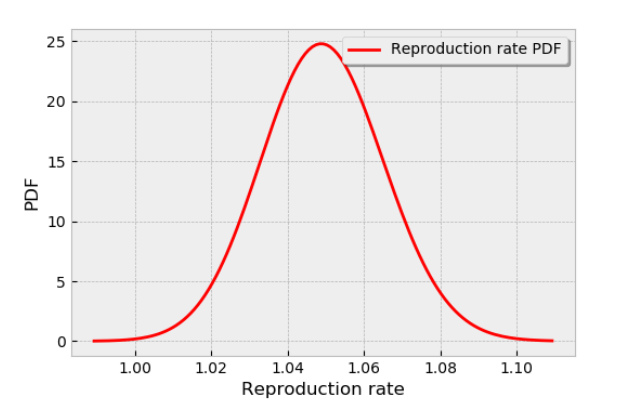
\includegraphics[width=0.5\linewidth]{r0.png}
  \caption{Densité de probabilité du taux de reproduction du virus. Cette loi visiblement normale a pour moyenne $1.04928$ et pour écart type $0.0160945$. Il y a de très fortes chances que le virus continue sa propagation, ce qui a effectivement été observé au Cameroun après le 14 juin 2020.}
  \label{fig:pdf}
\end{figure}

Pour une prédiction plus ambitieuse, nous proposons de faire une simulation pour prédire l'état des différentes groupes 15 jours après la fin de notre fenêtre d'étude (du 06 mars au 14 juin 2020). En d'autres termes, nous prédisons l'état de la population Camerounaise le 29 juin 2020. On obtient la figure ci-bas.  
\begin{figure}[H]
  \centering
  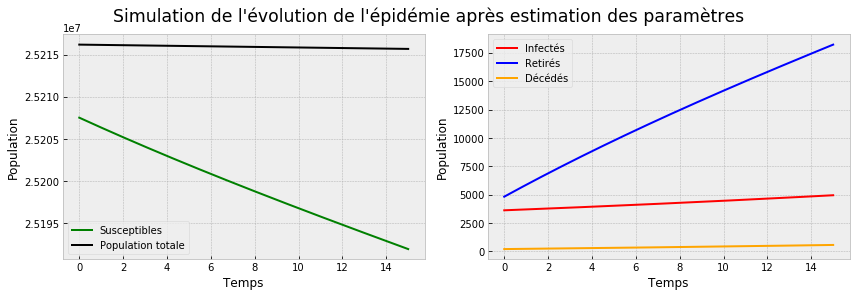
\includegraphics[width=\linewidth]{predict.png}
  \caption{Prédiction de l'état de la population Camerounaise le 29 juin 2020. Les populations sont séparées en deux figures en raison des échelles de grandeurs très différentes. Cette simulation correspond effectivement à une très bonne approximation de ce qui a été observé au Cameroun à la date indiquée. En effet, partant de $S_0,I_0,R_0,D_0=25207556,3633,4836, 212$ le 14 juin 2020, nous avons prédit $S_{pred},I_{pred},R_{pred},D_{pred}=25191938,4962,18251,576$ ; et les quantités $S_{true},I_{true},R_{true},D_{true}=25203645,2179,10100,313$ ont été observées. Naturellement, une prédiction plus loin dans le temps produit des résultats moins précis.}
  \label{fig:predict}
\end{figure}

%----------------------------------------------------------------------------------------
%	ASSIGNMENT CONTENT - SECTION 4
%----------------------------------------------------------------------------------------
\section*{Conclusion}

En conclusion, nous avons étudié l'évolution du COVID-19 au Cameroun à travers un modèle SIRD incluant les taux de natalité et de mortalité de la population. L'analyse de sensibilité qui en découle a montré que le nombre de décès est influencé par plusieurs paramètres, ce qui indique que les autorités ont plusieurs options pour minimiser les dégâts liés à ce virus. Notre étude s'est focalisée sur la fenêtre du 06 mars au 14 juin 2020, durant laquelle l'épidémie sévissait à grande ampleur. Nous pourrions étendre cette étude avec des estimations et des prédictions de l'évolution de l'épidémie durant la période actuelle de calme relatif (septembre 2020-janvier 2021). On pourrait par exemple rechercher la date à laquelle l'épidémie va s'achever\footnote{Tout ceci est possible dans le code de calcul qui est fournie nommé "Code.ipynb" ; il suffit juste de changer la date de début de l'étude et la duré de l'étude à l'endroit indiqué.}. Idéalement, il faudrait rechercher la loi de probabilité des différents paramètres en fonction du temps et des mesures de limitations appliquées par les gouvernements.     

% %-------------------------------------------------------------------------------
% %							THE BIBLIOGRAPHY
% %-------------------------------------------------------------------------------
\clearpage   % Pour retirer les references de la bare de navigation
% \cite{CNRS} \cite{Kaggle} \cite{GitHub} \cite{JHU} \cite{Nguemdjo}
\printbibliography


\end{document}
